% Options for packages loaded elsewhere
\PassOptionsToPackage{unicode}{hyperref}
\PassOptionsToPackage{hyphens}{url}
\PassOptionsToPackage{dvipsnames,svgnames,x11names}{xcolor}
%
\documentclass[
  letterpaper,
  DIV=11,
  numbers=noendperiod]{scrartcl}

\usepackage{amsmath,amssymb}
\usepackage{iftex}
\ifPDFTeX
  \usepackage[T1]{fontenc}
  \usepackage[utf8]{inputenc}
  \usepackage{textcomp} % provide euro and other symbols
\else % if luatex or xetex
  \usepackage{unicode-math}
  \defaultfontfeatures{Scale=MatchLowercase}
  \defaultfontfeatures[\rmfamily]{Ligatures=TeX,Scale=1}
\fi
\usepackage{lmodern}
\ifPDFTeX\else  
    % xetex/luatex font selection
\fi
% Use upquote if available, for straight quotes in verbatim environments
\IfFileExists{upquote.sty}{\usepackage{upquote}}{}
\IfFileExists{microtype.sty}{% use microtype if available
  \usepackage[]{microtype}
  \UseMicrotypeSet[protrusion]{basicmath} % disable protrusion for tt fonts
}{}
\makeatletter
\@ifundefined{KOMAClassName}{% if non-KOMA class
  \IfFileExists{parskip.sty}{%
    \usepackage{parskip}
  }{% else
    \setlength{\parindent}{0pt}
    \setlength{\parskip}{6pt plus 2pt minus 1pt}}
}{% if KOMA class
  \KOMAoptions{parskip=half}}
\makeatother
\usepackage{xcolor}
\setlength{\emergencystretch}{3em} % prevent overfull lines
\setcounter{secnumdepth}{-\maxdimen} % remove section numbering
% Make \paragraph and \subparagraph free-standing
\ifx\paragraph\undefined\else
  \let\oldparagraph\paragraph
  \renewcommand{\paragraph}[1]{\oldparagraph{#1}\mbox{}}
\fi
\ifx\subparagraph\undefined\else
  \let\oldsubparagraph\subparagraph
  \renewcommand{\subparagraph}[1]{\oldsubparagraph{#1}\mbox{}}
\fi


\providecommand{\tightlist}{%
  \setlength{\itemsep}{0pt}\setlength{\parskip}{0pt}}\usepackage{longtable,booktabs,array}
\usepackage{calc} % for calculating minipage widths
% Correct order of tables after \paragraph or \subparagraph
\usepackage{etoolbox}
\makeatletter
\patchcmd\longtable{\par}{\if@noskipsec\mbox{}\fi\par}{}{}
\makeatother
% Allow footnotes in longtable head/foot
\IfFileExists{footnotehyper.sty}{\usepackage{footnotehyper}}{\usepackage{footnote}}
\makesavenoteenv{longtable}
\usepackage{graphicx}
\makeatletter
\def\maxwidth{\ifdim\Gin@nat@width>\linewidth\linewidth\else\Gin@nat@width\fi}
\def\maxheight{\ifdim\Gin@nat@height>\textheight\textheight\else\Gin@nat@height\fi}
\makeatother
% Scale images if necessary, so that they will not overflow the page
% margins by default, and it is still possible to overwrite the defaults
% using explicit options in \includegraphics[width, height, ...]{}
\setkeys{Gin}{width=\maxwidth,height=\maxheight,keepaspectratio}
% Set default figure placement to htbp
\makeatletter
\def\fps@figure{htbp}
\makeatother

\usepackage{booktabs}
\usepackage{longtable}
\usepackage{array}
\usepackage{multirow}
\usepackage{wrapfig}
\usepackage{float}
\usepackage{colortbl}
\usepackage{pdflscape}
\usepackage{tabu}
\usepackage{threeparttable}
\usepackage{threeparttablex}
\usepackage[normalem]{ulem}
\usepackage{makecell}
\usepackage{xcolor}
\usepackage[auth-lg]{authblk}
\KOMAoption{captions}{tableheading}
\makeatletter
\makeatother
\makeatletter
\makeatother
\makeatletter
\@ifpackageloaded{caption}{}{\usepackage{caption}}
\AtBeginDocument{%
\ifdefined\contentsname
  \renewcommand*\contentsname{Table of contents}
\else
  \newcommand\contentsname{Table of contents}
\fi
\ifdefined\listfigurename
  \renewcommand*\listfigurename{List of Figures}
\else
  \newcommand\listfigurename{List of Figures}
\fi
\ifdefined\listtablename
  \renewcommand*\listtablename{List of Tables}
\else
  \newcommand\listtablename{List of Tables}
\fi
\ifdefined\figurename
  \renewcommand*\figurename{Figure}
\else
  \newcommand\figurename{Figure}
\fi
\ifdefined\tablename
  \renewcommand*\tablename{Table}
\else
  \newcommand\tablename{Table}
\fi
}
\@ifpackageloaded{float}{}{\usepackage{float}}
\floatstyle{ruled}
\@ifundefined{c@chapter}{\newfloat{codelisting}{h}{lop}}{\newfloat{codelisting}{h}{lop}[chapter]}
\floatname{codelisting}{Listing}
\newcommand*\listoflistings{\listof{codelisting}{List of Listings}}
\makeatother
\makeatletter
\@ifpackageloaded{caption}{}{\usepackage{caption}}
\@ifpackageloaded{subcaption}{}{\usepackage{subcaption}}
\makeatother
\makeatletter
\@ifpackageloaded{tcolorbox}{}{\usepackage[skins,breakable]{tcolorbox}}
\makeatother
\makeatletter
\@ifundefined{shadecolor}{\definecolor{shadecolor}{rgb}{.97, .97, .97}}
\makeatother
\makeatletter
\makeatother
\makeatletter
\makeatother
\ifLuaTeX
  \usepackage{selnolig}  % disable illegal ligatures
\fi
\IfFileExists{bookmark.sty}{\usepackage{bookmark}}{\usepackage{hyperref}}
\IfFileExists{xurl.sty}{\usepackage{xurl}}{} % add URL line breaks if available
\urlstyle{same} % disable monospaced font for URLs
\hypersetup{
  pdftitle={Modelos Lineares Generalizados Mistos},
  pdfauthor={Laíza Mendes - 20/0067028; César Augusto Galvão - 19/0011572},
  colorlinks=true,
  linkcolor={blue},
  filecolor={Maroon},
  citecolor={Blue},
  urlcolor={Blue},
  pdfcreator={LaTeX via pandoc}}

\title{Modelos Lineares Generalizados Mistos}
\usepackage{etoolbox}
\makeatletter
\providecommand{\subtitle}[1]{% add subtitle to \maketitle
  \apptocmd{\@title}{\par {\large #1 \par}}{}{}
}
\makeatother
\subtitle{Modelos Lineares Generalizados - 2/2023}
\author{Laíza Mendes - 20/0067028 \and César Augusto Galvão -
19/0011572}
\date{}

\begin{document}
\maketitle
\ifdefined\Shaded\renewenvironment{Shaded}{\begin{tcolorbox}[sharp corners, enhanced, boxrule=0pt, frame hidden, breakable, interior hidden, borderline west={3pt}{0pt}{shadecolor}]}{\end{tcolorbox}}\fi

\renewcommand*\contentsname{Table of contents}
{
\hypersetup{linkcolor=}
\setcounter{tocdepth}{3}
\tableofcontents
}
\newpage{}

\hypertarget{introduuxe7uxe3o}{%
\section{Introdução}\label{introduuxe7uxe3o}}

Em diversas áreas do conhecimento, pesquisas são feitas buscando uma
descrição de efeito em uma unidade de análise, porém com dados coletados
não apenas no nível da unidade. Muitas vezes, é de interesse compreender
como características de agrupamentos das unidades de análise interferem
no comportamento de interesse. Naturalmente, uma interpretação que surge
é de níveis de hierarquia das características estudadas, de modo que
modelos \emph{hierarquizados} ou \emph{multinível} são adequados para o
estudo do fenômeno.

Para dar concretude, pode-se pensar em um estudo sobre o desempenho
acadêmico de alunos. Para selecionar a amostra, escolas são amostradas
primeiro, em seguida turmas e, em um terceiro nível, alunos. Variáveis
como orçamento da escola, tempo de experiência dos professores das
turmas e renda familiar dos alunos são observadas. O pressuposto por
trás de um estudo com esse desenho é de que o desempenho dos alunos pode
ser afetado por características suas (renda familiar), da turma
(professor) e da escola (orçamento) de formas diferentes. Além disso, é
esperado que alunos da mesma turma tenham comportamentos correlacionados
e o mesmo pode ser esperado para turmas dentro da mesma escola.

Estudar de forma hierarquizada esse tipo de fenômeno permite evitar
falácias na modelagem devido à perda de poder da análise ou influência
exagerada de algumas variáveis devido à agregação ou desagregação de
variáveis de níveis hierárquicos diferentes. Além disso, é possível
estudar como agrupamentos das unidades de análise se comportam e como
isso influencia níveis inferiores da hierarquia.

Nessa classe de modelos é possível ter três combinações de tipos de
parâmetros:

\begin{enumerate}
\def\labelenumi{\arabic{enumi}.}
\tightlist
\item
  Todos os parâmetros são fixos, quando se tem um modelo de efeitos
  fixos;
\item
  Parte dos parâmetros é fixa e parte é aleatória, quando se tem um
  \textbf{modelo misto}; e
\item
  Todos os parâmetros são aleatórios, quando se tem um modelo aleatório.
\end{enumerate}

O foco deste trabalho são os modelos que pertencem ao tipo 2.

\newpage{}

\hypertarget{muxe9todo}{%
\section{Método}\label{muxe9todo}}

\hypertarget{modelagem}{%
\subsection{Modelagem}\label{modelagem}}

O modelo linear generalizado misto realizado neste relatório é ilustrado
a seguir. Considere uma amostra de tamanho \(n\) distribuída em \(J\)
agrupamentos em um modelo com apenas dois níveis de hierarquia. A
variável resposta
\(Y_{ij} \sim \text{Bernoulli}(p), \,\, i = 1, 2, \dots, n, \,\, j = 1, 2, \dots, J, \,\, 0 < p < 1\)
é uma variável binária e apenas uma covariável para cada nível de
hierarquia serão consideradas por simplicidade. Essas serão denotadas
por \(X\) e \(Z\) para a covariável de nível inferior e superior,
respectivamente.

O modelo com todos os parâmetros aleatórios pode ser genericamente
expresso da seguinte forma:

\begin{align}
  Y_{ij} = \beta_{0j} + \beta_{1j}X_{1ij} + \varepsilon_{ij}, \label{01}
\end{align}

em que \(\beta_{0j}\) é o intercepto para o grupo \(j\), \(\beta_{1j}\)
é o coeficiente geral para a covariável de nível hierárquico inferior
\(X_{1ij}\) e \(\varepsilon_{ij}\) é o elemento estocástico associado
associado à observação \(Y_{ij}\).

No entanto, para cada valor \(j\) o intercepto e o coeficiente são
influenciados também pelo comportamento das categorias de nível
hierárquico superior. É possível então expressá-los na forma

\begin{align}
  \beta_{0j} & = \gamma_{00} + \gamma_{01}Z_{j} + u_{0j}, \label{02} \\
  \beta_{1j} & = \gamma_{10} + \gamma_{11}Z_{j} + u_{1j}. \label{03}
\end{align}

Neste caso, \(\gamma_{(.)0}\) é o intercepto para \(\beta_{(.)j}\),
\(\gamma_{(.)1}\) é o coeficiente associado à covariável de nível
hierárquico superior \(Z_j\) para cada \(\beta_{(.)j}\) e \(u_{(.)j}\) é
o erro residual associado a cada \(\beta_{(.)j}\), ou seja, é associado
à dispersão entre as categorias de agrupamento\footnote{Em um modelo
  misto, bastaria escolher ou o intercepto ou o coeficiente, neste caso
  simplificado, como um termo que não varie em \(j\).}.

Finalmente, se substituimos (\ref{02}) e (\ref{03}) em (\ref{01}),
obtemos um detalhamento do modelo genérico em termos de suas componentes
hierarquizadas:

\begin{align}
  Y_{ij} = \gamma_{00} + \gamma_{01}Z_{j} + \gamma_{10}X_{1ij} + \gamma_{11}Z_{j}X_{1ij} + u_{1j}X_{1ij} + \varepsilon_{ij} + u_{0j}. \label{04}
\end{align}

Podemos interpretar as componentes da seguinte forma:

\begin{itemize}
\tightlist
\item
  Existe um intercepto geral -- \(\gamma_{00}\);
\item
  Existem efeitos que agem exclusivamente nas variáveis de um nível
  hierárquico específico -- \(\gamma_{01}Z_{j}\) e
  \(\gamma_{10}X_{1ij}\);
\item
  Existe um efeito de \emph{mediação} do comportamento do grupo sobre a
  unidade de observação -- \(\gamma_{11}Z_{j}X_{1ij}\);
\item
  Existem uma componente de variância do grupo que incide sobre o
  comportamento da unidade -- \(u_{1j}X_{1ij}\); e
\item
  Existem componentes de variância entre unidades e entre grupos --
  \(\varepsilon_{ij}\) e \(u_{0j}\) respectivamente.
\end{itemize}

As variâncias do modelo são obtidas de \(\varepsilon_{ij}\), \(u_{0j}\)
e \(u_{1j}\), assumidos como variáveis aleatórias Normais centradas em
zero, de modo que se pode calcular a proporção de variância no segundo
nível da hierarquia, entre agrupamentos. Essa medida é chamada de
correlação intraclasse e é dada por

\begin{align}
  \rho = \frac{\sigma^2_{u_0}}{\sigma^2_{u_0}+\sigma^2_{\varepsilon}+u_{1j}}.
\end{align}

No caso do modelo linear generalizado, especificamente o logístico, o
lado direito da equação (\ref{04}) é tomado como o preditor linear
\(\eta\) e a função de ligação adotada é a logit. Dessa forma, tem-se a
variável resposta \(Y\sim \text{Bin}(n,p), \,\, \mu = np\) e uma
candidata a função de ligação \(\eta = \text{logit}(\mu)\).

\hypertarget{estimauxe7uxe3o-e-testes-de-hipuxf3tese}{%
\subsection{Estimação e testes de
hipótese}\label{estimauxe7uxe3o-e-testes-de-hipuxf3tese}}

Entre os métodos de estimação comuns dos coeficientes do modelo, os
autores da referência principal deste relatório indicam maxima
verossimilhança restrita (REML), mínimos quadrados generalizados (GLS),
equações estimadoras generalizadas (GEE), bootstrap e métodos
bayesianos. No entanto, a documentação do pacote \texttt{lme4} para R
indica que, para a função \texttt{lme4::glmer()}, é utilizada quadratura
adaptativa de Gauss-Hermite para aproximação da log-verossimilhança.

Para a realização de testes de hipótese, assume-se que os estimadores
têm distirbuição normal e podem ser testados quanto à sua significância
usando teste de Wald.

Para conclusões sobre a eficácia do modelo, há diversas propostas como
os R quadrados de Cox e Snell ou o de Nagelkerke, explorado durante a
disciplina de MLG. No entanto, há uma extensão para modelos multinível
proposta por McKelvey e Zavoina (1975, \emph{apud} Moerbeek e Schoot,
2017) análogo ao \(R^2\). Ainda se atendo a um modelo simplificado de
dois níveis, a proporção de variância explicada pelo modelo pode ser
dada por

\begin{align}
    R^2_{MZ} = \frac{\sigma^2_{F}}{\sigma^2_{F}+\sigma^2_{u0}+\sigma^2_{R}},
\end{align}

onde \(\sigma^2_{F}\) é a variância do preditor linear,
\(\sigma^2_{uo}\) é a variância do intercepto e \(\sigma^2_{R}\) é a
variância do resíduo de nível mais baixo.

\hypertarget{resuxedduos}{%
\subsection{Resíduos}\label{resuxedduos}}

Resíduos em modelos multinível podem ser explorados de diversas formas
para verificar linearidade, homocedasticidade, autocorrelação, entre
outros. Uma das principais diferenças em relação a modelos não
hierarquizados é que há um resíduo para cada efeito aleatório no modelo.

Entre as formas de avaliação gráfica dos resíduos, pode-se citar:

\begin{itemize}
\tightlist
\item
  Resíduos padronizados versus escores da distribuição Normal;
\item
  Resíduos dos diferentes níveis versus a variável resposta;
\item
  Gráfico simultâneo da regressão para todas as classes estudadas;
\end{itemize}

\hypertarget{banco-de-dados}{%
\subsection{Banco de dados}\label{banco-de-dados}}

A título de ilustrar os métodos de modelagem para análise apresentados
acima, foi escolhido um banco de dados utilizado também no livro de
referência. Esse banco é sobre a educação na Tailândia e são orginados
de um estudo sobre o ensino pré-primário na Tailândia (Raudenbush \&
Bhumirat, 1992; see Raudenbush et al., 2004, p.~115). Nesse caso, temos
dois níveis claros presentes, o superior, que seria a escola, e o
inferior, que seriam os alunos.

Para a nossa análise, usaremos como variável resposta a variável REPEAT,
que é uma variável dicotômica que indica se o aluno repetiu ou não
alguma vez durante o ensino pré-primário, sendo, nos dados, 0 para não e
1 para sim. Além disso, há as variáveis usadas como explicativas para o
nível dos alunos, que seriam SEX, para expressar o sexo dos alunos (0
para menina e 1 para menino), e PPED, para sinalizar se o aluno teve ou
não educação pré-primária (0 para não e 1 para sim). Já para o nível das
escolas, foi utilizada a variável MSESC como variável preditora, ela
disgnifica a média SES que é a média dp índice socioeconômico associado
região onde se encontra a escola.

Fazendo uma análise descritiva inicial do banco de dados, notou-se que,
de um total de 441 escolas, somando 8582 alunos, 55 escolas apresentavam
a variável MSESC como NAs. Como essa é a única variável preditora das
escolas, para que fosse ilustrada corretamente a modelagem, foi
necessário retirá-las dos dados. Poderiam ser utilizadas algumas outras
alternativas estatísticas, mas decidimos apenas remover essas escolas da
análise, uma vez que, além do banco permanecer bem grande, com 7516
alunos, o foco da análise é apenas demonstrar, vide aplicação, os
conceitos vistos nesse trabalho para modelos multinível(ou modelos de
regressão hierárquica).

\hypertarget{pacotes-e-funuxe7uxf5es}{%
\subsection{Pacotes e funções}\label{pacotes-e-funuxe7uxf5es}}

Para o processo de modelagem, foi utilizado o pacote \texttt{lme4},
dedicado a modelos multinível. Deste pacote, a função \texttt{glmer()}
foi utilizada para computação dos modelos, isso porque essa função que é
usada para ajustar modelos lineares mistos generalizados quando a
variável de resposta é discreta, no nosso caso é binária, ou quando a
distribuição de erros não é normal.

\newpage{}

\hypertarget{resultados}{%
\section{Resultados}\label{resultados}}

\hypertarget{anuxe1lise-dos-possuxedveis-modelos}{%
\subsection{Análise dos possíveis
modelos}\label{anuxe1lise-dos-possuxedveis-modelos}}

Inicialmente, como análises anteriores a aplicação do banco de dados, é
importante testar se há ou não correlação entre as variáveis do banco.
Isso porque é necessário verificar se há multicolinearidade, uma vez que
essa interfere na eficiência do modelo. Logo, obteve-se

\begin{figure}

{\centering 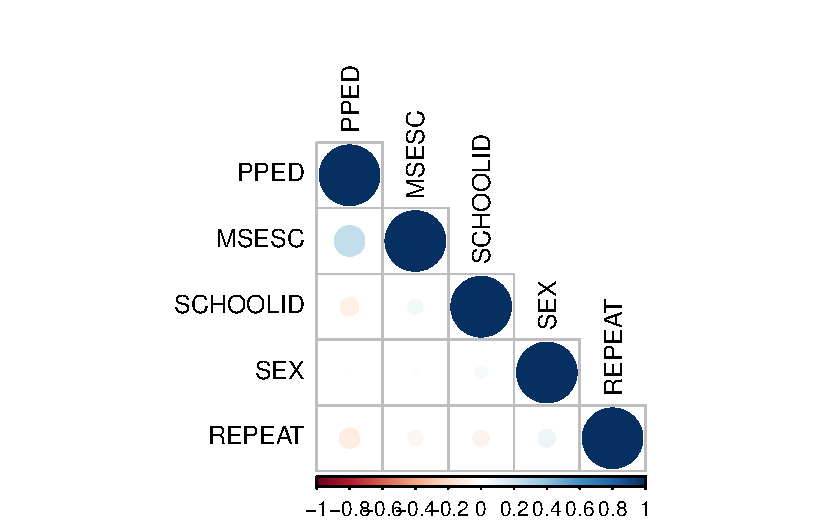
\includegraphics[width=0.8\textwidth,height=\textheight]{trabalho-final_files/figure-pdf/unnamed-chunk-1-1.pdf}

}

\end{figure}

Nota-se que as variáveis apresentam correlação muito baixa entre elas,
portanto, a multicolinearidade não é um problema para esses dados.

Para o banco de dados tratado, aplicamos 3 modelos, os quais comparamos
e analisamos qual de fato se ajustou melhor aos dados, foram eles:

\begin{itemize}
\item
  Modelo nulo: um modelo com o intercepto apenas, o mais simples
  possível, utilizado de base para avaliar se a inclusão de variáveis
  explicativas melhora significativamente o ajuste do modelo;
\item
  Modelo com variáveis explicativas fixas: um modelo com todas as
  variáveis explicativas do nível inferior fixas, incluindo SEX e PPED,
  assumindo que o efeito dessas variáveis é constante para todas as
  escolas, tendo efeitos aleatórios apenas no intercepto, em que
  poderemos entender o impacto mais direto dessas variáveis de nível
  inferior quanto a variável REPEAT;
\item
  Modelo hierárquico com efeitos aleatórios misto: um modelo que inclui
  a variáveil explicativa MSESC do nível superior, introduzindo efeitos
  aleatórios não só para o intercepto, mas também para a variável MSESC
  com relação a cada escola (nível superior).
\end{itemize}

Com isso, analisaremos qual dos três modelos se ajusta melhor aos dados
e se incluir variáveis explicativas, bem como incluir o efeito aleatório
para uma delas, fará diferença no que diz espeito a qualidade dos
modelos.

\hypertarget{modelo-nulo}{%
\subsubsection{Modelo nulo}\label{modelo-nulo}}

Partindo para a modelagem, começando pelo modelo nulo, obtemos os
seguintes resultados do resumo do modelo:

\begin{verbatim}
Generalized linear mixed model fit by maximum likelihood (Laplace
  Approximation) [glmerMod]
 Family: binomial  ( logit )
Formula: REPEAT ~ 1 + (1 | SCHOOLID)
   Data: dados_spss

     AIC      BIC   logLik deviance df.resid 
  5547.0   5560.8  -2771.5   5543.0     7514 

Scaled residuals: 
    Min      1Q  Median      3Q     Max 
-1.6295 -0.4173 -0.2480 -0.1755  4.7976 

Random effects:
 Groups   Name        Variance Std.Dev.
 SCHOOLID (Intercept) 1.668    1.292   
Number of obs: 7516, groups:  SCHOOLID, 356

Fixed effects:
              Estimate Std. Error z value Pr(>|z|)    
(Intercept) -2.2343255  0.0003828   -5836   <2e-16 ***
---
Signif. codes:  0 '***' 0.001 '**' 0.01 '*' 0.05 '.' 0.1 ' ' 1
optimizer (Nelder_Mead) convergence code: 0 (OK)
Model failed to converge with max|grad| = 0.184618 (tol = 0.002, component 1)
Model is nearly unidentifiable: very large eigenvalue
 - Rescale variables?
\end{verbatim}

Nota-se, do \textit{output} do código, que o modelo, que inclui apenas o
intercepto para cada nível da escola, apresenta intercepto é
estatisticamente significativo, em que quando todas as outras variáveis
são mantidas constantes, o log-odds de REPEAT para o grupo de referência
é \({-2.2343255}\). Dessa forma, há uma maior probabilidade média ou
chance de REPEAT ser igual a 0 (não ocorrer) em comparação com REPEAT
ser igual a 1 (ocorrer), em que a chance de repetir é \(e^{-2.2343255}\)
vezes a chance de não repetir. Além disso, nota-se que há também uma
variação significativa entre as escolas na interceptação do efeito médio
da resposta REPEAT.

\hypertarget{modelo-com-variuxe1veis-explicativas-fixas}{%
\subsubsection{Modelo com variáveis explicativas
fixas}\label{modelo-com-variuxe1veis-explicativas-fixas}}

Para esse modelo, acrescentamos as variáveis explicativas do nível dos
estudantes, ou seja, SEX e PPED. Elas serão colocadas no modelo como
variáveis fixas, em que não há efeito aleatório, dessa forma, obtemos

\begin{verbatim}
Generalized linear mixed model fit by maximum likelihood (Laplace
  Approximation) [glmerMod]
 Family: binomial  ( logit )
Formula: REPEAT ~ SEX + PPED + (1 | SCHOOLID)
   Data: dados_spss

     AIC      BIC   logLik deviance df.resid 
  5456.9   5484.6  -2724.4   5448.9     7512 

Scaled residuals: 
    Min      1Q  Median      3Q     Max 
-2.1587 -0.4039 -0.2474 -0.1679  6.1366 

Random effects:
 Groups   Name        Variance Std.Dev.
 SCHOOLID (Intercept) 1.634    1.278   
Number of obs: 7516, groups:  SCHOOLID, 356

Fixed effects:
            Estimate Std. Error z value Pr(>|z|)    
(Intercept) -2.23410    0.10054 -22.222  < 2e-16 ***
SEX          0.53494    0.07539   7.095 1.29e-12 ***
PPED        -0.64189    0.09860  -6.510 7.51e-11 ***
---
Signif. codes:  0 '***' 0.001 '**' 0.01 '*' 0.05 '.' 0.1 ' ' 1

Correlation of Fixed Effects:
     (Intr) SEX   
SEX  -0.440       
PPED -0.406 -0.002
optimizer (Nelder_Mead) convergence code: 0 (OK)
unable to evaluate scaled gradient
Model failed to converge: degenerate  Hessian with 2 negative eigenvalues
\end{verbatim}

todas as variaveis são estatisticamente significativas para o modelo.
Sendo o intercepto o log-odds de repetição para os alunos quando todas
as variáveis explicativas (SEX e PPED) são zero, como ele é igual a
-2.23410 nesse modelo, e é negativo, a chance de repetir é menor que a
de não repetir, ou seja, a chance de repetir é \(e^{-2.23410}\) vezes a
chance de não repetir. Ademais, quanto ao SEX, mantendo as outras
variáveis igual a 0, se ele aumenta em uma unidade (ou seja, quando muda
de ``girl'', 0, para ``boy'',1), a log-odds de repetição aumenta em
0.53494 vezes, então, a chance de repetir é e\^{}0.53494 vezes maior
para meninos. Em contrapartida, quando PPED aumenta em uma unidade, para
as outras variáveis iguais a 0 (ou seja, quando muda de ``não'' para
``sim'', teve educação pré primaria), a log-odds de repetição diminui em
0.64189 vezes, pois é negativo, logo, a chance de repetir é
\(e^-0.64189\) vezes a de não repetir para quem teve educação pré
primária.

\hypertarget{modelo-hieruxe1rquico-com-efeitos-aleatuxf3rios-misto}{%
\subsubsection{Modelo hierárquico com efeitos aleatórios
misto}\label{modelo-hieruxe1rquico-com-efeitos-aleatuxf3rios-misto}}

Por fim, para esse modelo adicionamos a variável preditora do nível da
escola, MSESC, em que agora, há um efeito aleatório da mesma sobre o
fator de cada variável explicativa em relação à variável resposta. Nessa
perspectiva, tem-se

\begin{verbatim}
Generalized linear mixed model fit by maximum likelihood (Laplace
  Approximation) [glmerMod]
 Family: binomial  ( logit )
Formula: REPEAT ~ SEX + PPED + (1 + MSESC | SCHOOLID)
   Data: dados_spss

     AIC      BIC   logLik deviance df.resid 
  5457.8   5499.3  -2722.9   5445.8     7510 

Scaled residuals: 
    Min      1Q  Median      3Q     Max 
-2.3829 -0.4021 -0.2467 -0.1714  6.0794 

Random effects:
 Groups   Name        Variance Std.Dev. Corr 
 SCHOOLID (Intercept) 1.454    1.206         
          MSESC       1.154    1.074    -0.38
Number of obs: 7516, groups:  SCHOOLID, 356

Fixed effects:
            Estimate Std. Error z value Pr(>|z|)    
(Intercept) -2.24718    0.10607 -21.186  < 2e-16 ***
SEX          0.53496    0.07591   7.047 1.83e-12 ***
PPED        -0.64527    0.09915  -6.508 7.61e-11 ***
---
Signif. codes:  0 '***' 0.001 '**' 0.01 '*' 0.05 '.' 0.1 ' ' 1

Correlation of Fixed Effects:
     (Intr) SEX   
SEX  -0.432       
PPED -0.395 -0.004
\end{verbatim}

Assim, a análise fica análoga a do modelo anterior com relação a PPED,
SEX e o intercepto, a diferença é que agora, como MSESC está imbutido em
SCHOOLID (MSESC) dos efeitos aleatórios, ela indica que há uma variância
de 1.154 entre as escolas com relação ao MSESC.

\hypertarget{comparando-os-modelos}{%
\subsection{Comparando os modelos}\label{comparando-os-modelos}}

Diante dos três modelos acima, podemos fazer a escolha daquele que
melhor se adequa aos dados. Com isso, fez-se o teste de deviance por
meio da tabela ANOVA para comparar o modelo 1 com o modelo 2, obtendo-se
o seguinte resultado

\begin{verbatim}
Data: dados_spss
Models:
modelo_intercepto: REPEAT ~ 1 + (1 | SCHOOLID)
modelo_efeitos_fixos: REPEAT ~ SEX + PPED + (1 | SCHOOLID)
                     npar    AIC    BIC  logLik deviance  Chisq Df Pr(>Chisq)
modelo_intercepto       2 5547.0 5560.8 -2771.5   5543.0                     
modelo_efeitos_fixos    4 5456.9 5484.6 -2724.4   5448.9 94.088  2  < 2.2e-16
                        
modelo_intercepto       
modelo_efeitos_fixos ***
---
Signif. codes:  0 '***' 0.001 '**' 0.01 '*' 0.05 '.' 0.1 ' ' 1
\end{verbatim}

Considerando, para esse teste, \(H_0\) de que a inclusão de termos
adicionais no modelo 2 não melhora significativamente o ajuste do modelo
aos dados, e o modelo mais simples 1 é suficiente, pode-se afirmar que
há evidências de que o modelo 2 é mais adequado aos dados que o modelo
1.

Por conseguinte, comparamos o modelo 2 ao modelo 3, para verificar de
fato qual é o mais adequado. Assim, resulta-se na seguinte tabela ANOVA

\begin{verbatim}
Data: dados_spss
Models:
modelo_efeitos_fixos: REPEAT ~ SEX + PPED + (1 | SCHOOLID)
modelo_efeitos_aleatorios: REPEAT ~ SEX + PPED + (1 + MSESC | SCHOOLID)
                          npar    AIC    BIC  logLik deviance  Chisq Df
modelo_efeitos_fixos         4 5456.9 5484.6 -2724.4   5448.9          
modelo_efeitos_aleatorios    6 5457.8 5499.3 -2722.9   5445.8 3.0859  2
                          Pr(>Chisq)
modelo_efeitos_fixos                
modelo_efeitos_aleatorios     0.2137
\end{verbatim}

Como não rejeita-se H0 de que modelo mais simples é suficiente, em favor
do modelo mais complexo, não há evidências de que o modelo mais simples
não seja suficiente ou de que a inclusão do efeito aleatório da variável
MSESC de nível superior melhore significativamente o ajuste do modelo
aos dados.

\hypertarget{modelo-escolhido}{%
\subsection{Modelo escolhido}\label{modelo-escolhido}}

Diante dos resultados acima, vamos escolher o modelo mais completo, o
modelo 3, com a variável de nível superior MSESC, a fim de se obter
algumas estatisticas sobre o mesmo, inclusive para fazer a análise de
resíduos, já que nosso trabalho fala sobre modelos mistos, mesmo que não
haja de fato melhora estatisticamente significativa ao escolher esse
modelo em relação ao segundo modelo mostrado.

Calcularemos, então, a estatística da correlação intraclasse, que indica
quanto da variação total na variável resposta (REPEAT) pode ser
atribuída às diferenças entre as escolas. Assim, com uma correlação
intraclasse de 0.9378021, pode-se interpretar que, como está próximo de
1, a maior parte da variação na probabilidade de um aluno repetir ao
menos uma vez está relacionada às diferenças entre as escolas, ou
melhor, às diferenças socioeconômicas da região (MSESC). Isso sugere que
a variabilidade nessa probabilidade é significativamente influenciada
pela escola à qual os alunos pertencem.

\hypertarget{anuxe1lise-de-resuxedduos}{%
\subsection{Análise de Resíduos}\label{anuxe1lise-de-resuxedduos}}

Com isso, para o modelo escolhido, é de suma importância que seja feita
a análise dos resíduos para que seja garantida a eficiência do modelo.

Inicialmente, fazendo-se o teste de normalidade para os resíduos.

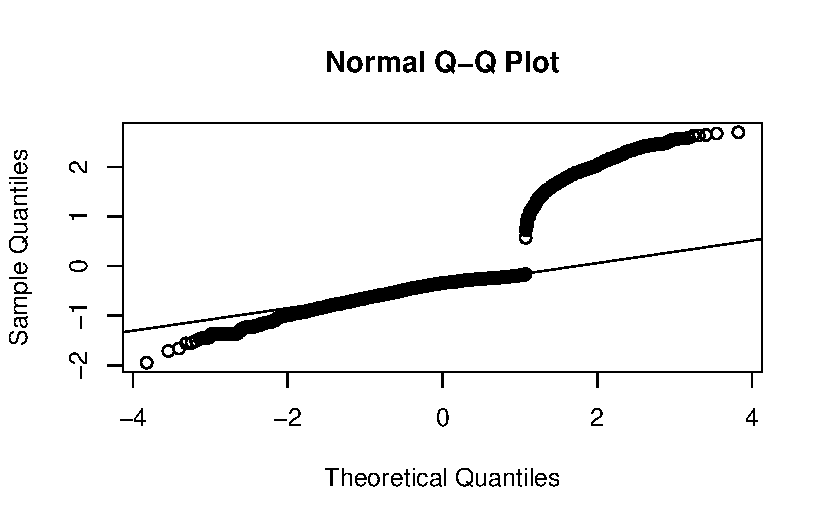
\includegraphics{trabalho-final_files/figure-pdf/unnamed-chunk-8-1.pdf}

Nota-se que os resíduos não são normais, o que faz sentido, dado o fato
de que a variável preditora é uma binomial.

\newpage{}

\hypertarget{discussuxe3o}{%
\section{Discussão}\label{discussuxe3o}}

Com uma finalidade exemplificativa, foi exposta superficialmente a
fundamentação teórica para modelos lineares generalizados multinível.
Além disso, foi selecionado um banco de dados utilizado pelos autores da
principal referência deste relatório para demonstrar a aplicação do
modelo.

Para demonstrar o processo de modelagem, foram ajustados três modelos:
um modelo nulo, outro com efeitos fixos e um terceiro com efeitos
mistos. Não foram encontradas diferenças significativas de deviance
entre os três, mas foi mantida a análise dos efeitos mistos com
propósitos pedagógicos. Dessa forma, o modelo de efeitos mistos, mesmo
não apresentando uma significativa melhoria em termos de explicação da
variância em relação ao modelo nulo, apresentou todos os coeficientes
significativamente diferentes de zero.

Uma das dificuldades encontradas foi conseguir identificar todos os
coeficientes do modelo utilizando o output do R. Dessa forma, não
conseguimos expressar o modelo obtido em uma expressão algébrica em sua
forma completa. Outra dificuldade encontrada foi identificar teoria e
funções que realizasse medidas diagnósticas de influência como DFFIT,
DFBETAS, COVRatio, entre outros. Como não foram identificadas, não foi
feita análise de pontos de influência.

\newpage{}

\hypertarget{apuxeandice}{%
\section{Apêndice}\label{apuxeandice}}

A principal referência utilizada neste trabalho foram os capítulos 1, 2,
3, 4 e 6 de Hox, J., Moerbeek, M., \& Van de Schoot, R. (2017).
\emph{Multilevel analysis: Techniques and applications}. Routledge.

Todo o projeto de composição deste documento pode ser encontrado aqui:
\url{https://github.com/cesar-galvao/Listas-MLG/tree/main/trabalho_final}



\end{document}
